\documentclass[11pt]{article}

\usepackage[margin=0.92in]{geometry}
\usepackage[T1]{fontenc}
\usepackage{newtxtext,newtxmath}
\usepackage{microtype}
\usepackage{amsmath,mathtools,bm}
\usepackage{booktabs,tabularx,array}
\usepackage{enumitem}
\usepackage{graphicx}
\usepackage{tikz}
\usetikzlibrary{arrows.meta,positioning,calc,fit}
\usepackage{natbib}
\usepackage{caption}
\usepackage{float}
\usepackage{placeins}
\usepackage{hyperref}
\usepackage{xurl}

\hypersetup{
  hidelinks,
  pdfauthor={Rajeev Yadav, Ph.D.},
  pdftitle={Validation-Gated Adaptive Probabilistic Forecasting in Nonstationary Equity Markets}
}

\setlength{\parindent}{1.15em}
\setlength{\parskip}{0pt}
\setlength{\emergencystretch}{2em}
\setlist[itemize]{leftmargin=1.6em,itemsep=0.15em,topsep=0.25em}
\setlist[enumerate]{leftmargin=1.7em,itemsep=0.15em,topsep=0.25em}
\captionsetup{font=small,labelfont=bf}
\renewcommand{\arraystretch}{1.12}

\newcommand{\sigmoid}{\operatorname{sigmoid}}
\newcommand{\logit}{\operatorname{logit}}
\newcommand{\clip}{\operatorname{clip}}
\newcommand{\E}{\mathbb{E}}
\newcommand{\Var}{\operatorname{Var}}
\newcommand{\Prb}{\mathbb{P}}
\newcommand{\I}{\mathbb{I}}
\newcommand{\R}{\mathbb{R}}
\newcommand{\calF}{\mathcal{F}}
\newcommand{\calJ}{\mathcal{J}}
\newcommand{\version}{1.0.0}

\title{\textbf{Validation-Gated Adaptive Probabilistic Forecasting\\in Nonstationary Equity Markets}}
\author{Rajeev Yadav, Ph.D.\\\texttt{rajeevyadav@gmail.com}}
\date{August 2026}

\begin{document}
\maketitle

\begin{abstract}
A probability forecast in a financial market is a claim about an event that has not yet occurred, made with information that was available at a particular time. That simple statement creates several practical difficulties. Financial labels overlap, company information arrives asynchronously, macroeconomic series are revised, the same data are often examined repeatedly, and a model that was calibrated during development may become unreliable after deployment. This paper develops a forecasting architecture in which those difficulties are part of the model specification rather than after-the-fact warnings. Three quantities are kept separate. The first is a Bayesian evidence score used for interpretable research triage; its uncertainty concerns the score itself and is not a return probability. The second is a frozen empirical probability of a fixed forward excess-return event. It is trained with point-in-time inputs, purge-and-embargo rules, separated calibration and stacking stages, and a locked test set. The third is a bounded online Bayesian residual that reacts to new market, filing, and macroeconomic information while leaving the validated anchor unchanged. Online parameters are updated only after the original forward outcome has matured. The adaptive correction is applied only after date-balanced prequential loss, calibration, temporal breadth, and drift conditions are satisfied. The paper develops the model from first principles, then gives the full mathematical specification, including fractional-Beta evidence aggregation, Bayesian logistic inference with a Laplace approximation, constrained probabilistic stacking, dependence-aware bootstrap validation, freshness decay, sequential rank-one covariance updating, and fail-closed deployment logic. Synthetic fixtures are used only to test the statistical machinery and software invariants. They are explicitly not evidence of market forecasting skill.
\end{abstract}

\noindent\textbf{Keywords:} probabilistic forecasting; Bayesian logistic regression; online learning; calibration; prequential evaluation; temporal leakage; concept drift; point-in-time data; financial machine learning.

\section{Introduction}

Suppose a forecasting system assigns a stock a probability of $0.58$ of outperforming a benchmark over the next year. At noon the company files a material report, the stock gaps relative to the benchmark, and credit spreads move at the same time. There are two unsatisfactory ways to react. A purely static model ignores the information until the next scheduled retraining. An uncontrolled online model can react immediately, but it can also begin ``learning'' from the new observation before the one-year outcome is known. The first approach is slow; the second can quietly destroy the meaning of the original validation.

The practical question is therefore not simply how to predict. It is how to change a probability when the information set changes, without pretending that the future label has already arrived. A second question follows immediately: how should a forecasting system demonstrate that its probabilities deserve to be interpreted as probabilities rather than as scores with a percent sign attached?

These questions are unusually difficult in financial data. The signal-to-noise ratio is low, many observations share the same market environment, long-horizon labels overlap, and researchers can test many alternatives on the same finite history. The probability of obtaining an apparently attractive backtest therefore increases with repeated experimentation, even when no stable economic relation has been found. This problem has been studied from several directions, including data snooping, multiple testing and backtest overfitting \citep{white2000reality,harvey2016crosssection,bailey2017pbo}. Temporal leakage adds another layer: if an observation dated $t$ uses a filing, revision or price that was not actually knowable at $t$, the backtest is no longer a historical simulation of the information available to the forecaster.

The approach developed here is conservative by construction. It separates three statistical objects that are often mixed together in financial applications. A research score summarizes current evidence and carries uncertainty about that score. A frozen anchor model estimates an empirical forward-event probability and is not changed casually after validation. A third model learns a bounded residual correction from newly arriving information. The residual may alter a candidate probability immediately, but its coefficients are updated only when the corresponding outcome has matured. If the online layer has too little temporal evidence, poor calibration, worse proper scores, stale inputs, or a drift alert, the system falls back to the frozen anchor.

The distinction matters. A statement such as ``there is a high posterior probability that the research score exceeds 8'' is not the same statement as ``there is a 64\% probability that the stock will outperform.'' The former is uncertainty about an internally defined score. The latter is an empirical forecasting claim that must be calibrated against realized events. Keeping these claims apart is the starting point of the model.

The reference implementation used to make the discussion concrete is FinCompass v\version. The software is not the contribution by itself. It is useful here because every equation in the paper is tied to an executable rule, a validation gate, or an audit artifact. The bundled models and data fixtures remain classified as synthetic regression fixtures; no bundled model is represented as a validated market forecaster.

\subsection{How to read the paper}

The paper is written in layers. Sections 2--4 can be read without a background in Bayesian statistics. They define the event being forecast and explain why the three probabilities must remain separate. Sections 5--10 give the full statistical model and validation protocol. Sections 11--13 deal with online activation, drift, lineage and reproducibility. The appendices collect derivations and implementation defaults for readers who want to reproduce the calculations exactly.

\section{What does a financial probability mean?}
\label{sec:meaning}

A useful probability forecast must answer three questions: what event is being forecast, what information was available when the forecast was made, and how often similar probabilities have been correct in held-out data. Without those three pieces, a number between zero and one is not yet a defensible probability forecast.

Let $i$ denote a security, $b$ a benchmark, and $t$ an observation time. Let $\calF_t$ denote all information available to the system at time $t$. A valid feature vector $X_{i,t}$ must be measurable with respect to $\calF_t$; informally, every input must have been knowable at the time of the forecast.

For a horizon of $H$ common trading sessions, define the stock and benchmark returns
\begin{align}
R_{i,t}^{(H)} &= \frac{P_i(\tau_H(t))}{P_i(t)}-1, \\
R_{b,t}^{(H)} &= \frac{P_b(\tau_H(t))}{P_b(t)}-1,
\end{align}
where $\tau_H(t)$ is the $H$th trading session on which both the stock and benchmark have a usable price after $t$. For an excess-return hurdle $\eta$, the binary event is
\begin{equation}
Y_{i,t}^{(H,\eta)}
=\I\left\{R_{i,t}^{(H)}-R_{b,t}^{(H)}>\eta\right\}.
\label{eq:target}
\end{equation}
The strict reference configuration uses $H=252$, benchmark SPY, and $\eta=0$.

Equation~\eqref{eq:target} is more important than it may first appear. The outcome is not ``whatever happened about a year later.'' It is attached to a precise endpoint. If the background process that resolves labels is delayed by two weeks, the target does not move by two weeks. Let
\begin{equation}
\mathcal T_{i,b}(t)=\{u_1<u_2<\cdots\}
\end{equation}
be the ordered common trading sessions after $t$. Then
\begin{equation}
\tau_H(t)=u_H.
\label{eq:exactendpoint}
\end{equation}
A label is not available until $u_H$ exists, and once it exists the endpoint is $u_H$, not the date on which a scheduler happens to run.

The corresponding forecasting probability is
\begin{equation}
p_{i,t}=\Prb\left(Y_{i,t}^{(H,\eta)}=1\mid\calF_t\right).
\label{eq:probdef}
\end{equation}
A model may estimate this probability badly, of course, but Equation~\eqref{eq:probdef} states what the number is intended to mean.

\subsection{A small numerical example}

Consider an anchor probability $p^A=0.58$. Its log-odds are
\begin{equation}
\logit(0.58)=\log\frac{0.58}{0.42}\approx0.323.
\end{equation}
Suppose new information produces a validated residual correction of $0.33$ in log-odds units. The candidate probability is then
\begin{equation}
p^C=\sigmoid(0.323+0.33)\approx0.658.
\end{equation}
The candidate has moved from 58\% to about 65.8\%. But this does not imply that the residual model is allowed to control the live output. If the online validation gate is still warming up, the live probability remains $0.58$. The event can change the candidate belief now; the system learns from whether that belief was useful only after the future outcome becomes observable.

This simple example contains most of the architecture. The rest of the paper makes each step precise.

\section{Three statistical objects, not one}
\label{sec:three}

The architecture is easiest to understand if the three outputs are named before the mathematics is introduced.

The \emph{evidence score} is a 0--10 research summary built from profitability, durability, safety, valuation and current-regime evidence. Its posterior distribution expresses uncertainty about that score. It is not trained to match frequencies of future outperformance.

The \emph{anchor probability} is an empirical model of Equation~\eqref{eq:target}. It is trained on historical observations that respect point-in-time availability and is frozen after validation. It can be live only if its data and locked-test results satisfy a defined governance tier.

The \emph{adaptive probability} starts from the anchor and applies a bounded residual in log-odds space using fresh market, filing and macroeconomic information. The residual has its own posterior state, performance history and activation gate.

Figure~\ref{fig:architecture} shows the separation. The arrows indicate permissible information flow; they do not imply that every plane is eligible for live use.

\begin{figure}[H]
\centering
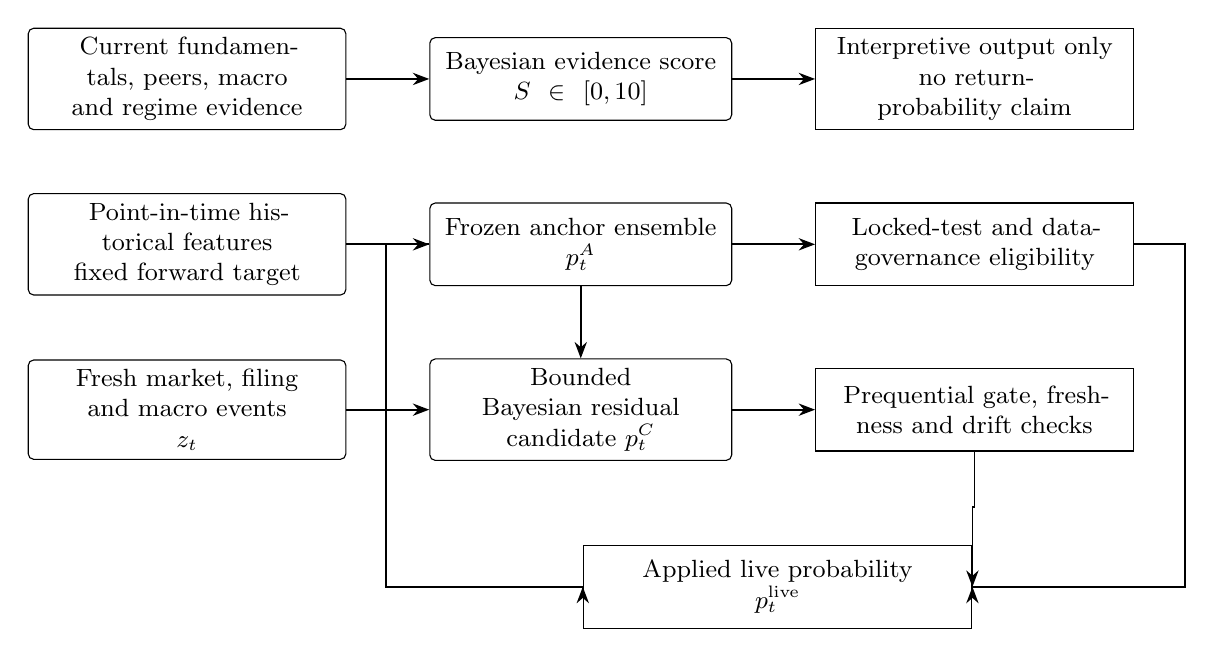
\begin{tikzpicture}[
  >=Stealth,
  every node/.style={font=\small},
  source/.style={draw, rounded corners=2pt, align=center, text width=3.8cm, minimum height=1.05cm},
  model/.style={draw, rounded corners=2pt, align=center, text width=3.6cm, minimum height=1.05cm},
  rule/.style={draw, align=center, text width=3.8cm, minimum height=1.05cm},
  arr/.style={->, line width=0.65pt}
]
\node[source] (es) at (0,2.8) {Current fundamentals, peers, macro and regime evidence};
\node[model] (em) at (5.0,2.8) {Bayesian evidence score\\$S\in[0,10]$};
\node[rule] (er) at (10.0,2.8) {Interpretive output only\\no return-probability claim};

\node[source] (as) at (0,0.7) {Point-in-time historical features\\fixed forward target};
\node[model] (am) at (5.0,0.7) {Frozen anchor ensemble\\$p_t^A$};
\node[rule] (ar) at (10.0,0.7) {Locked-test and data-governance eligibility};

\node[source] (rs) at (0,-1.4) {Fresh market, filing and macro events\\$z_t$};
\node[model] (rm) at (5.0,-1.4) {Bounded Bayesian residual\\candidate $p_t^C$};
\node[rule] (rr) at (10.0,-1.4) {Prequential gate, freshness and drift checks};

\node[rule, text width=4.7cm] (live) at (7.5,-3.65) {Applied live probability\\$p_t^{\mathrm{live}}$};

\draw[arr] (es)--(em); \draw[arr] (em)--(er);
\draw[arr] (as)--(am); \draw[arr] (am)--(ar);
\draw[arr] (rs)--(rm); \draw[arr] (rm)--(rr);
\draw[arr] (am.south) -- (rm.north);
\draw[arr] (rr.south) -- ++(0,-0.70) -| (live.east);
\draw[arr] (ar.east) -- ++(0.65,0) -- ++(0,-4.35) -| (live.east);
\draw[arr] (am.west) -- ++(-0.55,0) -- ++(0,-4.35) -| (live.west);
\end{tikzpicture}
\caption{Separation of the three statistical objects. The evidence score, frozen empirical probability, and online residual have different meanings and different activation rules.}
\label{fig:architecture}
\end{figure}

A common failure in financial software is to collapse these layers. A high research score is relabeled as a high probability of return, or a live price shock is fed into a model that was validated only on end-of-day data. The present architecture prohibits both operations unless the corresponding probability model has been validated for the claimed information contract.

\section{Point-in-time information and the avoidance of hindsight}
\label{sec:pit}

The phrase \emph{point in time} means more than attaching a date to a row. A historical observation should contain only values that a forecaster could have possessed on that date.

For an accounting item whose fiscal period ends at $q$, let $a(q)$ be its public availability time. The item is eligible for a feature vector observed at time $t$ only when
\begin{equation}
a(q)\le t.
\label{eq:availability}
\end{equation}
Joining fundamentals by fiscal period end alone can therefore create hindsight. A March quarter that was filed in May must not appear in an April observation.

The same issue occurs in macroeconomic data. Many series are revised. A backtest that fills every historical date with the latest revised value uses information that did not exist in real time. Vintage-aware databases such as ALFRED are designed precisely to distinguish the value known today from the value known at an earlier real-time date \citep{fred_realtime}. For company filings, the SEC disseminates submission information throughout the day; in the live layer, the acceptance timestamp is used when available, with the filing date only as a fallback \citep{sec_edgar_api}.

Prices require their own discipline. The anchor model retains the same daily feature semantics used during its validation. An intraday quote is not substituted into a daily feature merely because the quote is newer. Intraday information belongs to the separately validated residual layer.

The point-in-time contract can be summarized by one rule: if the historical version of the system could not have known a value at $t$, the value does not belong in $X_{i,t}$.

\section{The evidence plane: uncertainty about a research score}
\label{sec:evidence}

The first plane is deliberately simpler than the forecasting model. It answers a research question: given the evidence presently available, how strong is the company-and-regime profile under a transparent scoring rubric, and how uncertain is that score because evidence is incomplete?

This plane uses five pillars: quality, financial durability, safety, valuation and current cycle/regime context. Each raw metric is first mapped to a continuous 0--10 scale. The continuity matters because a company with a return on invested capital of 11.99\% should not receive a materially different score from an otherwise identical company at 12.01\% merely because a hand-built bin boundary was crossed.

\subsection{Continuous metric maps}

Suppose metric $x$ is represented by ordered scoring knots $(a_k,s_k)$, where $a_k$ is a raw metric value and $s_k\in[0,10]$. Between adjacent knots, the score is linearly interpolated:
\begin{equation}
f(x)=s_k+\frac{x-a_k}{a_{k+1}-a_k}(s_{k+1}-s_k),
\qquad a_k\le x\le a_{k+1}.
\label{eq:interp}
\end{equation}
Values beyond the outer knots are clipped to the endpoint scores. The function $f$ is chosen to be economically monotone over the region where such monotonicity is defensible.

When a sufficiently large sector peer sample is available, the absolute score can be supplemented with a robust relative measure. Let $m_j$ and $\operatorname{IQR}_j$ be the peer median and interquartile range for metric $j$. Define
\begin{equation}
z_j^{\mathrm{IQR}}=d_j\frac{x_j-m_j}{\max(\operatorname{IQR}_j,\varepsilon)},
\end{equation}
where $d_j=1$ when larger values are preferable and $d_j=-1$ when smaller values are preferable. The peer score is
\begin{equation}
s_j^{\mathrm{peer}}=\clip\left(5+2.2z_j^{\mathrm{IQR}},1,9.5\right).
\end{equation}
With peer weight $\rho$, the metric score is
\begin{equation}
s_j=(1-\rho)s_j^{\mathrm{abs}}+\rho s_j^{\mathrm{peer}}.
\label{eq:peerblend}
\end{equation}
The default implementation uses $\rho=0.25$ for the general case, with small variations for specific metrics. If fewer than five suitable peers are available, the relative term is omitted instead of being estimated from an unstable sample.

\subsection{Why a Beta model appears here}

The 0--10 score can be normalized as $q_j=s_j/10$. This is not a Bernoulli observation in a literal frequentist sense. It is fractional evidence on a bounded scale. A Beta distribution is useful because it provides a transparent way to accumulate such evidence while shrinking sparse pillars toward a neutral prior.

For pillar $r$, let $\calJ_r$ be the available metrics and let $w_j$ be their evidence weights. Starting from prior $\operatorname{Beta}(\alpha_0,\beta_0)$, the fractional update is
\begin{align}
\alpha_r &= \alpha_0+c\sum_{j\in\calJ_r}w_jq_j,\\
\beta_r  &= \beta_0+c\sum_{j\in\calJ_r}w_j(1-q_j),
\label{eq:betaupdate}
\end{align}
where $c$ controls the strength assigned to one unit of rubric evidence. The default prior is neutral, $\alpha_0=\beta_0=2$, and the implementation uses $c=4$.

If $U_r\sim\operatorname{Beta}(\alpha_r,\beta_r)$, the reported pillar score is
\begin{equation}
S_r=10\E[U_r]=10\frac{\alpha_r}{\alpha_r+\beta_r}.
\label{eq:pillarscore}
\end{equation}
The posterior variance is
\begin{equation}
\Var(U_r)=\frac{\alpha_r\beta_r}{(\alpha_r+\beta_r)^2(\alpha_r+\beta_r+1)}.
\label{eq:betavar}
\end{equation}
When little evidence is present, the posterior remains close to the neutral prior and its interval remains broad. With more consistent evidence, the posterior moves away from five and becomes narrower. This is the desired behavior: missing data reduce confidence rather than being silently replaced by favorable assumptions.

Evidence coverage is reported separately. If $W_r^{\mathrm{obs}}$ is the sum of observed metric weights and $W_r^{\mathrm{exp}}$ is the expected weight under the pillar definition, then
\begin{equation}
C_r=\min\left(1,\frac{W_r^{\mathrm{obs}}}{W_r^{\mathrm{exp}}}\right).
\end{equation}
A score of 8 with low coverage is therefore distinguishable from a score of 8 supported by a nearly complete evidence set.

\subsection{Composite uncertainty and overlapping pillars}

Let $\lambda_r$ be the fixed pillar weights, with $\sum_r\lambda_r=1$. A naive composite draw would be
\begin{equation}
S^{(m)}=10\sum_r\lambda_rU_r^{(m)}.
\label{eq:composite}
\end{equation}
The difficulty is that the pillars are not independent. Quality and durability can share profitability evidence, and cycle context can reuse valuation or capital-return information. Treating all pillar posteriors as independent would make the composite interval artificially narrow.

Rather than inventing an empirical covariance matrix that has not been estimated, the implementation propagates two dependence scenarios. In the first, pillar draws are independent. In the second, the marginal draws are sorted and paired by rank, creating a comonotonic, perfectly positively dependent scenario. If $[L_{\mathrm{ind}},U_{\mathrm{ind}}]$ and $[L_{\mathrm{com}},U_{\mathrm{com}}]$ are the corresponding 90\% intervals, the reported model interval is the envelope
\begin{equation}
[L,U]=\left[\min(L_{\mathrm{ind}},L_{\mathrm{com}}),\ 
\max(U_{\mathrm{ind}},U_{\mathrm{com}})\right].
\label{eq:depenvelope}
\end{equation}
This is a sensitivity analysis, not a claim that the real dependence is comonotonic. Its purpose is to prevent a convenient independence assumption from communicating more precision than the evidence supports.

The current-regime pillar also carries a causal guardrail. It may use valuation regime, capital-return quality, yield-curve slope, high-yield spreads and commodity context, but it is described only as current regime evidence. It is not interpreted as a recession timer or a forward return forecast. That distinction is enforced in the user-facing explanation and by regression tests in the reference implementation.

\section{The frozen anchor: an empirical forward-event model}
\label{sec:anchor}

The anchor is the first plane that is allowed to make the probability claim in Equation~\eqref{eq:probdef}. It is not derived from the 0--10 evidence posterior. It is fitted to labeled historical events.

The reference ensemble contains three deliberately different learners: Bayesian logistic regression, histogram gradient boosting, and a regularized random forest. The logistic component provides interpretable posterior coefficient uncertainty. The two tree-based models allow nonlinearities and interactions that a single linear log-odds surface cannot capture. The models are calibrated separately, combined with nonnegative weights, and calibrated once more at the ensemble level.

\subsection{Bayesian logistic component}

Let $x_n\in\R^p$ be a feature vector and $y_n\in\{0,1\}$ its target. With an intercept included in $x_n$, the logistic model is
\begin{equation}
\Prb(Y_n=1\mid x_n,\beta)=\sigmoid(x_n^\top\beta),
\qquad
\sigmoid(a)=\frac{1}{1+e^{-a}}.
\label{eq:logistic}
\end{equation}
A zero-centered Gaussian prior is placed on the coefficients,
\begin{equation}
\beta\sim\mathcal N(0,\sigma_\beta^2I).
\label{eq:prior}
\end{equation}
The strict default uses $\sigma_\beta=1.5$ after the feature preprocessing defined by the model pipeline.

Ignoring constants, the log posterior is
\begin{equation}
\ell(\beta)
=\sum_{n=1}^{N}\left[y_n\log p_n+(1-y_n)\log(1-p_n)\right]
-\frac{1}{2\sigma_\beta^2}\beta^\top\beta,
\label{eq:logpost}
\end{equation}
where $p_n=\sigmoid(x_n^\top\beta)$. The maximum a posteriori estimate $\hat\beta$ maximizes Equation~\eqref{eq:logpost}. The negative Hessian at the mode is
\begin{equation}
H=X^\top W X+\sigma_\beta^{-2}I,
\qquad
W=\operatorname{diag}\{p_n(1-p_n)\}.
\label{eq:hessian}
\end{equation}
A Laplace approximation gives
\begin{equation}
\beta\mid\mathcal D\approx\mathcal N(\hat\beta,H^{-1}).
\label{eq:laplace}
\end{equation}
Posterior coefficient draws can then be propagated through Equation~\eqref{eq:logistic} to obtain a coefficient-uncertainty interval for the logistic component \citep{mackay1992bayesian}.

The interval is useful but should not be oversold. It conditions on the chosen model family and training data; it does not include every form of model misspecification, structural break, or market uncertainty.

\subsection{Nonlinear components and component calibration}

The histogram gradient-boosting and random-forest components are standard probabilistic classifiers \citep{friedman2001greedy,breiman2001random}. Their raw class probabilities are not assumed to be calibrated. Each component is therefore mapped through a calibration function using a chronologically later validation stage.

For sigmoid calibration, a convenient form is
\begin{equation}
C(p)=\sigmoid\{a\,\logit(p)+b\}.
\label{eq:sigcal}
\end{equation}
The implementation also supports isotonic calibration, a monotone nonparametric mapping, but the strict reference profile uses sigmoid calibration. Calibrators are fit without using the locked test set \citep{niculescu2005predicting,gneiting2007calibration}.

\subsection{Constrained probabilistic stacking}

Let $\tilde p_{nk}$ be the calibrated probability from component $k$ for validation observation $n$. The uncalibrated ensemble probability is
\begin{equation}
q_n=\sum_{k=1}^{K}w_k\tilde p_{nk},
\qquad
w_k\ge0,\quad\sum_{k=1}^{K}w_k=1.
\label{eq:stack}
\end{equation}
The weights are selected on a separate chronological validation stage by minimizing a regularized Brier objective,
\begin{equation}
\hat w
=\arg\min_{w\in\Delta_K}
\left\{
\frac{1}{N}\sum_{n=1}^{N}(q_n-y_n)^2
+\lambda\sum_{k=1}^{K}\left(w_k-\frac1K\right)^2
\right\},
\label{eq:stackopt}
\end{equation}
where $\Delta_K$ is the probability simplex and the implementation uses $\lambda=0.01$. A final calibrator $C_E$ is fitted on a third chronological validation stage:
\begin{equation}
p_n^A=C_E(q_n).
\label{eq:anchorprob}
\end{equation}
This separation is intentional. If component calibration, stacking and final calibration are optimized on the same observations, the reported calibration can be better than the procedure deserves.

\section{Temporal validation: why random holdout is not enough}
\label{sec:temporal}

A conventional random train/test split assumes that observations can be exchanged without changing the problem. Long-horizon financial labels violate that assumption. If forecasts are sampled monthly but evaluated one year ahead, neighboring observations share much of the same future return path. Securities observed on the same date also share market conditions.

The validation design therefore has two jobs: prevent information from crossing chronological boundaries and preserve enough dependence in uncertainty estimates that the effective sample size is not exaggerated.

\subsection{Purge and embargo}

Suppose a later partition begins at date $s$. A training observation at date $t$ is retained only if its target has fully resolved before $s$,
\begin{equation}
\tau_H(t)<s.
\label{eq:purge}
\end{equation}
An additional embargo of $E$ business days requires
\begin{equation}
t<s-\operatorname{BDay}(E).
\label{eq:embargo}
\end{equation}
The strict reference configuration uses $E=252$. These rules are applied not only between the broad train, validation and test partitions, but also between the three internal validation roles used for component calibration, stacking and final calibration.

Figure~\ref{fig:timeline} shows the order. The blank gaps are not wasted data. They are the cost of preventing forward target windows from straddling fitting boundaries.

\begin{figure}[H]
\centering
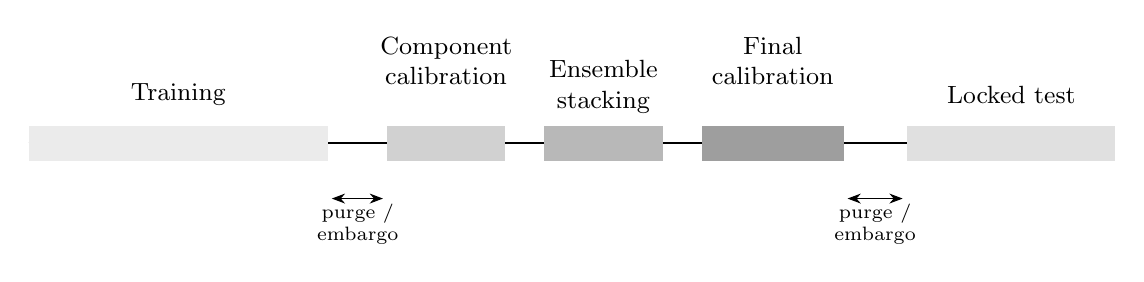
\begin{tikzpicture}[x=1cm,y=1cm,>=Stealth,every node/.style={font=\small}]
  \draw[line width=0.7pt] (0,0) -- (13.8,0);
  \fill[black!8] (0, -0.22) rectangle (3.8,0.22);
  \fill[black!18] (4.55,-0.22) rectangle (6.05,0.22);
  \fill[black!28] (6.55,-0.22) rectangle (8.05,0.22);
  \fill[black!38] (8.55,-0.22) rectangle (10.35,0.22);
  \fill[black!12] (11.15,-0.22) rectangle (13.8,0.22);

  \node[align=center] at (1.9,0.62) {Training};
  \node[align=center,text width=2.2cm] at (5.30,1.05) {Component\\calibration};
  \node[align=center,text width=2.0cm] at (7.30,0.72) {Ensemble\\stacking};
  \node[align=center,text width=2.1cm] at (9.45,1.05) {Final\\calibration};
  \node[align=center] at (12.48,0.62) {Locked test};

  \draw[<->] (3.85,-0.70) -- (4.50,-0.70);
  \node[align=center,font=\scriptsize] at (4.18,-1.03) {purge /\\embargo};
  \draw[<->] (10.40,-0.70) -- (11.10,-0.70);
  \node[align=center,font=\scriptsize] at (10.75,-1.03) {purge /\\embargo};
\end{tikzpicture}
\caption{Chronological development protocol. Internal calibration and stacking roles are separated in time, and the locked test is not used for model fitting or threshold selection.}
\label{fig:timeline}
\end{figure}

The locked test has a strict meaning: it is not used to choose features, hyperparameters, ensemble weights, calibration method, validation thresholds, or governance rules. If it is inspected repeatedly while those decisions are still changing, it is no longer a locked test. This is the same broad problem addressed by the backtest-overfitting literature: repeated search turns apparently out-of-sample evidence into another form of in-sample optimization \citep{bailey2017pbo}.

\subsection{Moving date-block and cross-sectional cluster bootstrap}

Even a clean locked test can understate uncertainty if its dependence structure is ignored. Let $d_1,\ldots,d_D$ denote the distinct observation dates in the test set, and let $\mathcal C(d)$ contain all securities observed on date $d$. The bootstrap samples contiguous blocks of observation dates and includes the entire cross-sectional cluster $\mathcal C(d)$ whenever date $d$ is selected.

If forecasts are sampled every $\Delta$ trading days and evaluated over $H$ trading days, the automatic block length is
\begin{equation}
L=\left\lceil\frac{H}{\Delta}\right\rceil.
\label{eq:blocklength}
\end{equation}
For $H=252$ and $\Delta=21$, $L=12$ observation dates. This combines the logic of block resampling for serial dependence with same-date clustering for market-wide dependence \citep{kunsch1989jackknife,politis1994stationary}. It does not prove that the bootstrap captures every dependence mechanism; it is a deliberately more conservative alternative to treating each row as an independent draw.

\section{How probabilistic forecasts are scored}
\label{sec:metrics}

Classification accuracy throws away most of the information in a probability. A forecast of $0.51$ and a forecast of $0.99$ produce the same class label if both are thresholded at 0.5, even though the second makes a much stronger claim. Proper scoring rules retain that distinction.

For observations $(p_n,y_n)$, the Brier score is
\begin{equation}
\operatorname{BS}=\frac1N\sum_{n=1}^{N}(p_n-y_n)^2,
\label{eq:brier}
\end{equation}
and binary log loss is
\begin{equation}
\operatorname{LL}=-\frac1N\sum_{n=1}^{N}
\left[y_n\log p_n+(1-y_n)\log(1-p_n)\right].
\label{eq:logloss}
\end{equation}
Both reward honest probability estimates and penalize confident errors \citep{brier1950verification,gneiting2007proper}.

A reference model uses an event rate estimated from development data, not from the locked test. For either score,
\begin{equation}
\operatorname{Skill}=1-\frac{\operatorname{Score}_{\mathrm{model}}}
{\operatorname{Score}_{\mathrm{reference}}}.
\label{eq:skill}
\end{equation}
Positive skill means the model improves on the constant-probability reference under that proper score.

Discrimination and calibration are checked separately. ROC AUC and average precision describe ranking behavior. Calibration asks whether events with forecast probability near $p$ occur at approximately frequency $p$. A calibration regression may be written
\begin{equation}
\logit\Prb(Y=1)=a+b\logit(p).
\label{eq:calslope}
\end{equation}
Ideal calibration corresponds to $a=0$ and $b=1$. Expected calibration error (ECE) gives a binned summary, but it must be interpreted with care because its value depends on binning and sample composition.

The strict fixture gate requires, among other conditions, positive Brier and log-loss skill, a minimum AUC, acceptable ECE and calibration slope, adequate class counts, enough locked-test dates and elapsed span, positive skill in a sufficient fraction of purged walk-forward folds, and dependence-aware bootstrap bounds that do not cross specified failure thresholds. A passing gate is evidence about a particular model, target, dataset and protocol. It is not a general certificate that the market relation will persist indefinitely.

\section{Anchor uncertainty: what is and is not covered}
\label{sec:anchoruncertainty}

The Bayesian logistic component provides a natural distribution over coefficients. The other components do not. The implementation therefore reports an \emph{uncertainty envelope}, not a formal predictive interval with guaranteed market coverage.

For each observation, Bayesian coefficient draws produce lower and upper logistic-component probabilities. These are calibrated. The ensemble also has calibrated component point probabilities from gradient boosting and random forest. The lower envelope is the minimum of the Bayesian lower bound and all component probabilities; the upper envelope is defined analogously. Because the final sigmoid or isotonic calibrator is monotone, the envelope endpoints can be passed through the final calibrator.

The result is useful for abstention and model-disagreement diagnostics, but its interpretation is deliberately narrow: it combines Bayesian coefficient uncertainty and inter-model dispersion. It does not integrate every uncertainty source in the data-generating process. In particular, it is not a prediction interval for a future return.

The reference implementation may abstain when the final probability lies sufficiently close to $0.5$ or when an interval rule configured by the user is triggered. Abstention is not a failure to predict; it is an explicit acknowledgement that a binary decision would be more precise than the model evidence warrants.

\section{The adaptive residual: reacting to new information}
\label{sec:adaptive}

A validated anchor should not be refitted every time new information appears. At the same time, a live system should not ignore a material filing or a large relative price move simply because the next full retraining is weeks away. The compromise used here is a residual model in log-odds space.

Let $p_t^A$ be the frozen anchor probability and let $z_t\in\R^{13}$ be the live feature vector. The adaptive coefficient state at time $t$ has posterior mean $m_t$ and covariance $P_t$. The raw residual is
\begin{equation}
\delta_t^{\mathrm{raw}}=z_t^\top m_t.
\label{eq:rawdelta}
\end{equation}
To prevent the residual from overwhelming the anchor, the log-odds shift is bounded:
\begin{equation}
\delta_t=\clip\left(\delta_t^{\mathrm{raw}},-d_{\max},d_{\max}\right).
\label{eq:boundedshift}
\end{equation}
The balanced reference profile uses $d_{\max}=0.75$. The candidate probability is
\begin{equation}
p_t^C=
\clip\left[
\sigmoid\left\{\logit(p_t^A)+\delta_t\right\},
\epsilon,1-\epsilon
\right],
\label{eq:candidate}
\end{equation}
with $\epsilon=0.01$ in the balanced profile.

There is a useful interpretation of the bound. Since odds are multiplied by $e^{\delta_t}$, the residual can change the anchor odds by at most
\begin{equation}
\exp(d_{\max})=\exp(0.75)\approx2.12
\end{equation}
in either direction before probability clipping. The online layer is therefore influential, but it is not allowed to erase the validated anchor in one step.

The posterior variance of the unbounded log-odds correction is
\begin{equation}
s_{\delta,t}^2=z_t^\top P_tz_t.
\label{eq:deltavar}
\end{equation}
This quantity is displayed as a state-uncertainty diagnostic. As with the anchor envelope, it should not be confused with a complete predictive distribution for market returns.

\subsection{The 13-dimensional live feature contract}

The implemented vector is
\begin{equation}
\begin{split}
z_t=(&r_{1d},\ r_{1d}^{\mathrm{rel}},\ z_{r,20},\ z_{r,20}^{\mathrm{rel}},\ z_{V,20},\ \mathrm{range}_{1d},\\
&f_{\mathrm{SEC}},\ f_{8K/6K},\ f_{10Q},\ f_{10K},\ \Delta YC,\ \Delta HY,\ f_{\mathrm{macro}})^\top.
\end{split}
\label{eq:featurevector}
\end{equation}
The first six features describe current market behavior. Four features represent the freshness and broad family of the most recent SEC filing. Two represent changes in the yield curve and high-yield spread. The final term measures macroeconomic freshness.

Table~\ref{tab:features} gives the contract in words. The feature names are intentionally modest. For example, a fresh 10-Q indicator says that a quarterly filing arrived recently; it does not claim that the filing is good or bad. A future extension may add validated textual or numerical event interpretation, but an external feed is context-only by default until separately validated.

\begin{table}[H]
\centering
\small
\caption{Adaptive feature vector used by the reference implementation.}
\label{tab:features}
\begin{tabularx}{\textwidth}{@{}>{\raggedright\arraybackslash}p{0.30\textwidth}X@{}}
\toprule
Feature & Interpretation \\
\midrule
Market return, 1 day & Previous session close to latest price; includes the overnight gap when available. \\
Benchmark-relative return, 1 day & Stock move minus benchmark move over the corresponding interval. \\
Return $z$-score, 20 & Standardized recent stock return shock. \\
Relative-return $z$-score, 20 & Standardized recent stock-minus-benchmark shock. \\
Volume $z$-score, 20 & Standardized unusual volume. \\
Intraday range & High-low range normalized by price. \\
SEC filing freshness & Exponentially decayed age of the most recent filing. \\
8-K/6-K, 10-Q, 10-K-family terms & Filing-family indicator multiplied by SEC freshness. \\
Yield-curve change & Recent curve change, freshness-weighted. \\
High-yield spread change & Recent spread change, freshness-weighted. \\
Macro freshness & Exponentially decayed age of the current macro observation. \\
\bottomrule
\end{tabularx}
\end{table}

\subsection{Freshness is different from event age}

A live system must distinguish an old event from an unverified source. If no new 10-Q has been filed for several weeks, the most recent filing is simply old. If the SEC source has not been successfully checked for several days, the system cannot know whether a newer filing was missed.

For a source event of age $a$ seconds and half-life $h$ hours, the freshness multiplier is
\begin{equation}
f(a;h)=\exp\left(-\log(2)\frac{a}{3600h}\right).
\label{eq:freshness}
\end{equation}
The balanced profile uses a 36-hour event half-life for SEC information and four times that half-life for macroeconomic event decay. Separately, each provider has a maximum allowed verification staleness. If the most recent successful provider check is older than that limit, source-dependent adaptive features are set to zero until verification resumes. Thus an old event decays; an unverified source is suppressed.

The polling scheduler uses the timestamp of the last provider check, not the timestamp of the last distinct event. Otherwise a provider that repeatedly reports ``nothing new'' could be polled on every browser refresh after the first cadence window.

\section{Online Bayesian learning, one matured label at a time}
\label{sec:online}

The adaptive model follows a predict-before-update rule. At observation time $t$, the system records $p_t^A$, $z_t$ and the candidate $p_t^C$. It does not yet know $Y_t$. The pending label is bound to the base model, benchmark, target definition, adaptive settings fingerprint and state lineage. Only when the exact endpoint in Equation~\eqref{eq:exactendpoint} is available is the outcome resolved and used for learning.

This ordering is a form of prequential evaluation: predict first, observe the outcome later, then update \citep{dawid1984prequential}. It prevents the model from evaluating a forecast with information obtained after the forecast was made.

\subsection{Dynamic prior between updates}

Let the posterior before a new matured observation be approximately
\begin{equation}
\theta_{t-1}\mid\mathcal D_{t-1}\approx\mathcal N(m_{t-1},P_{t-1}).
\end{equation}
Before incorporating the next label, uncertainty is inflated by a forgetting factor $\lambda_f\in(0,1]$ and process noise $q\ge0$:
\begin{equation}
P_t^-=\frac{P_{t-1}}{\lambda_f}+qI,
\qquad
m_t^-=m_{t-1}.
\label{eq:dynamicprior}
\end{equation}
The balanced profile uses $\lambda_f=0.997$ and $q=0.0005$. Old information is therefore discounted gradually rather than discarded abruptly. This is related to dynamic logistic models in which coefficients are allowed to evolve over time \citep{penny1999dynamic,mccormick2012dynamic}.

\subsection{Rank-one posterior update}

For the matured observation, let $z=z_t$ and let $p=p_t^C$ be the probability issued before learning from its label $y$. The local Bernoulli curvature is
\begin{equation}
w=p(1-p).
\end{equation}
Define
\begin{equation}
v=P_t^-z,
\qquad
d=1+wz^\top v.
\label{eq:vd}
\end{equation}
A one-step Gaussian/Laplace update is
\begin{align}
P_t &= P_t^- - \frac{w}{d}vv^\top,
\label{eq:rankonecov}\\
m_t &= m_t^- + \frac{v}{d}(y-p).
\label{eq:rankonemean}
\end{align}
Equation~\eqref{eq:rankonecov} is the Woodbury/Sherman-Morrison form of the inverse Hessian update. It avoids recomputing a matrix pseudoinverse for every matured label. With only 13 adaptive coefficients, either method is feasible in isolation, but the rank-one form is numerically cleaner and has bounded cost for continuous use. A small positive-definiteness floor is applied after symmetrization if numerical roundoff produces an eigenvalue too close to zero.

The initial residual mean is zero. Consequently, before any online learning, the candidate probability equals the anchor probability. The prior covariance is $\sigma_0^2I$, where the balanced profile uses $\sigma_0=0.75$.

\subsection{Why repeated screen refreshes do not create evidence}

A live application may display many predictions during one trading day. Those displays are not independent learning trials. The implementation permits frequent prediction refreshes but limits effective learning observations by ticker, model and observation date. More generally, the activation gate requires not only a minimum number of matured rows but also a minimum number of unique observation dates and a minimum elapsed calendar span.

This distinction becomes important in a large watchlist. Two hundred stocks observed on one date provide a large cross section but only one market date. They should not be mistaken for two hundred independent demonstrations that an online model is stable through time.

\section{Prequential activation: the adaptive model must earn control}
\label{sec:gate}

The online model is allowed to produce a candidate from the first observation, but it is not automatically allowed to replace the anchor in the live output. Activation depends on recent matured forecasts.

Let $\mathcal D$ be the set of observation dates in the evaluation window and let $n_d$ be the number of matured observations on date $d$. For a loss function $\ell$, the date-balanced loss is
\begin{equation}
\bar L
=\frac{1}{|\mathcal D|}
\sum_{d\in\mathcal D}
\frac{1}{n_d}\sum_{i=1}^{n_d}\ell(p_{di},y_{di}).
\label{eq:datebalancedloss}
\end{equation}
Every date receives the same total weight. This prevents a day with a large cross section from dominating the temporal evidence.

The same principle is used for online ECE. Give observation $(d,i)$ weight
\begin{equation}
\omega_{di}=\frac{1}{|\mathcal D|n_d}.
\label{eq:dateweight}
\end{equation}
For probability bin $B_k$, let $W_k=\sum_{(d,i)\in B_k}\omega_{di}$. Then
\begin{equation}
\operatorname{ECE}_{\mathrm{date}}
=\sum_k W_k\left|
\frac{\sum_{(d,i)\in B_k}\omega_{di}p_{di}}{W_k}
-
\frac{\sum_{(d,i)\in B_k}\omega_{di}y_{di}}{W_k}
\right|.
\label{eq:dateece}
\end{equation}
This is not a new universal definition of ECE. It is a governance metric chosen to keep online calibration from being dominated by the number of tickers sampled on a particular date.

For the balanced profile, the gate requires at least 120 matured observations, at least 60 unique observation dates, and at least 180 calendar days of span. It also requires the adaptive date-balanced Brier score and log loss to be no worse than the anchor under zero-regret thresholds, ECE no greater than 0.08, and no drift alert. Formally, with checks $G_1,\ldots,G_m$,
\begin{equation}
G_t=\bigwedge_{j=1}^{m}G_j.
\label{eq:gate}
\end{equation}
Only if $G_t=1$ and adaptive application is enabled may the residual control the live probability.

\section{Drift protection}
\label{sec:drift}

A model can pass an activation gate and later deteriorate. The online layer therefore compares its squared-error loss with the anchor on each matured observation. Define
\begin{equation}
e_t=(p_t^C-y_t)^2-(p_t^A-y_t)^2.
\label{eq:lossdiff}
\end{equation}
Positive $e_t$ means the adaptive model was worse on that observation. An exponentially weighted mean and variance are maintained:
\begin{align}
\mu_t&=(1-\alpha)\mu_{t-1}+\alpha e_t,\\
s_t^2&=(1-\alpha)s_{t-1}^2+\alpha(e_t-\mu_t)^2.
\label{eq:ewma}
\end{align}
After a minimum number of samples, an alert is raised when
\begin{equation}
\mu_t>a+c\frac{s_t}{\sqrt{n_t}},
\label{eq:driftalert}
\end{equation}
where $a$ is an allowance and $c$ is a control multiplier. The balanced profile uses $\alpha=0.08$, $a=0.001$, $c=2.75$, and a minimum of 60 samples.

This rule is a deterioration safeguard, not a formal hypothesis test with a claimed Type-I error rate. It borrows the practical logic of sequential control methods \citep{page1954continuous,roberts1959control}: persistent loss relative to the anchor is more important than one bad outcome. If the alert is active, the residual fails the gate and control returns to the anchor.

\section{The fail-closed live probability}
\label{sec:live}

The deployment rule can now be written compactly. Let $A_t$ indicate that a frozen anchor is eligible for live use under its governance tier. Let $G_t$ be the adaptive gate in Equation~\eqref{eq:gate}. Then
\begin{equation}
p_t^{\mathrm{live}}=
\begin{cases}
\text{unavailable}, & A_t=0,\\[3pt]
p_t^C, & A_t=1\ \text{and}\ G_t=1,\\[3pt]
p_t^A, & A_t=1\ \text{and}\ G_t=0.
\end{cases}
\label{eq:live}
\end{equation}
The adaptive layer therefore cannot promote an ineligible anchor. It can only modify an anchor that has already earned live eligibility. Likewise, a source outage does not cause the system to infer that ``nothing happened.'' Source-dependent residual features are suppressed when verification is stale.

Figure~\ref{fig:onlinecycle} shows the operational sequence for one forecast. Notice the long delay between prediction and learning when $H=252$.

\begin{figure}[H]
\centering
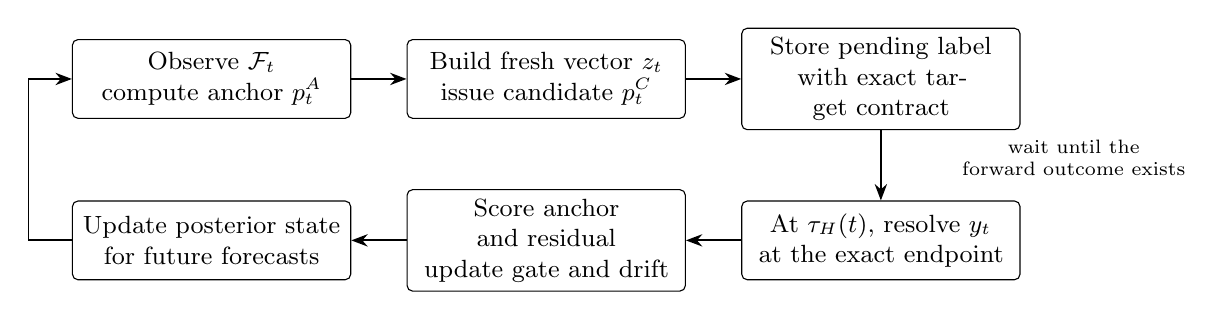
\begin{tikzpicture}[
  >=Stealth,
  every node/.style={font=\small},
  boxstep/.style={draw, rounded corners=2pt, align=center, text width=3.3cm, minimum height=1.0cm},
  arr/.style={->,line width=0.65pt}
]
\node[boxstep] (s1) at (0,0) {Observe $\calF_t$\\compute anchor $p_t^A$};
\node[boxstep] (s2) at (4.25,0) {Build fresh vector $z_t$\\issue candidate $p_t^C$};
\node[boxstep] (s3) at (8.50,0) {Store pending label\\with exact target contract};
\node[boxstep] (s4) at (8.50,-2.05) {At $\tau_H(t)$, resolve $y_t$\\at the exact endpoint};
\node[boxstep] (s5) at (4.25,-2.05) {Score anchor and residual\\update gate and drift};
\node[boxstep] (s6) at (0,-2.05) {Update posterior state\\for future forecasts};
\draw[arr] (s1)--(s2); \draw[arr] (s2)--(s3); \draw[arr] (s3)--(s4);
\draw[arr] (s4)--(s5); \draw[arr] (s5)--(s6);
\draw[arr] (s6.west) -- ++(-0.55,0) -- ++(0,2.05) -- (s1.west);
\node[font=\scriptsize,align=center] at (10.95,-1.0) {wait until the\\forward outcome exists};
\end{tikzpicture}
\caption{Predict-before-update cycle. New information can affect a candidate probability immediately; model learning occurs only after the original outcome has matured.}
\label{fig:onlinecycle}
\end{figure}

\section{Lineage, settings, and reproducibility}
\label{sec:lineage}

A configurable research platform creates a subtle statistical problem: changing a setting can change the meaning of a model. A 126-day target is not the same model as a 252-day target. A QQQ-relative event is not the same event as an SPY-relative event. A residual trained with a responsive forgetting factor is not the same posterior state as one trained under a conservative profile.

For this reason, settings that change the target or learning semantics are part of model identity. A frozen model manifest records the target, feature contract, data provenance, split dates, calibration method, validation metrics and artifact hash. The model identifier is bound to the serialized artifact hash.

The adaptive state key is derived from the base model identifier, adaptive engine version and a fingerprint of the complete adaptive settings contract. Pending labels carry the same lineage. If a user changes from one adaptive profile to another, the new profile begins or resumes its own compatible state; it does not reinterpret the old posterior under new process noise, forgetting, freshness or gate assumptions.

This design has a practical benefit. A future audit can answer not only ``what probability was shown?'' but also ``which target, model, settings, event state and validation tier produced it?'' Reproducibility is therefore treated as part of the statistical model rather than as an optional software feature.

\section{Validation tiers}
\label{sec:tiers}

Passing numerical thresholds is not sufficient to claim market validation if the dataset itself is biased. The reference implementation uses four tiers.

\begin{table}[H]
\centering
\small
\caption{Model governance tiers.}
\label{tab:tiers}
\begin{tabularx}{\textwidth}{@{}>{\raggedright\arraybackslash}p{0.22\textwidth}X@{}}
\toprule
Tier & Meaning \\
\midrule
\texttt{fixture\_only} & Synthetic or deterministic data used to verify software, statistics, leakage controls and release regression behavior. Never live-eligible. \\
\texttt{rejected} & Required statistical or data-governance conditions were not met. \\
\texttt{validated\_research} & The empirical model passed its locked-test gate on real historical data, but the dataset may still carry limitations that prevent the strongest market claim. \\
\texttt{validated\_market} & In addition to statistical gates, the dataset documents point-in-time features, historical-universe/survivorship control, delisted securities, and corporate-action-adjusted prices. \\
\bottomrule
\end{tabularx}
\end{table}

The distinction between \texttt{validated\_research} and \texttt{validated\_market} prevents a common shortcut: reporting excellent test metrics on a present-day universe and overlooking the securities that disappeared from that universe. Delisting bias can materially distort historical performance \citep{shumway1997delisting}.

\section{Synthetic regression results}
\label{sec:fixtures}

The bundled fixtures answer a narrow but useful question: if the statistical code is changed, do the expected temporal splits, calibration stages, bootstrap procedures, online updates and gates still behave as intended? They do not answer whether the model contains exploitable market signal.

\subsection{Frozen anchor fixture}

The deterministic anchor fixture contains 6,528 training observations, 1,920 validation observations and 2,304 locked-test observations. The test partition spans 72 observation dates over 1,988 calendar days. Table~\ref{tab:anchorresults} reports the locked-test metrics from the frozen reference artifact.

\begin{table}[H]
\centering
\small
\caption{Frozen-anchor locked-test regression metrics on the synthetic fixture.}
\label{tab:anchorresults}
\begin{tabular}{@{}lr@{}}
\toprule
Metric & Value \\
\midrule
Brier score & 0.217727 \\
Brier skill & 0.117815 \\
Log loss & 0.623959 \\
Log-loss skill & 0.091430 \\
ROC AUC & 0.699801 \\
Average precision & 0.623286 \\
ECE (10 bins) & 0.035934 \\
Calibration slope & 0.800691 \\
Calibration intercept & -0.081872 \\
Locked-test observations & 2,304 \\
Distinct test dates & 72 \\
\bottomrule
\end{tabular}
\end{table}

With the moving 12-date block/cross-sectional cluster bootstrap, the 90\% lower bound for Brier skill is 0.10898, the lower bound for log-loss skill is 0.08343, the lower bound for ROC AUC is 0.69373, and the upper bound for ECE is 0.04917. All four purged walk-forward folds have positive Brier skill; their median Brier skill is approximately 0.1303. The learned ensemble weights are approximately 0.4730 for Bayesian logistic regression, 0.2301 for histogram gradient boosting, and 0.2969 for random forest.

These values are deliberately easier to interpret than to market: they show that the fixture and validation machinery are internally consistent. Because the data are synthetic, none of the values is evidence that the same performance exists in real markets.

\subsection{Adaptive streaming fixture}

The adaptive fixture contains a 1,200-observation warm-up sequence followed by a 600-observation locked prequential stream. The model predicts before every update. The locked results are shown in Table~\ref{tab:adaptresults}.

\begin{table}[H]
\centering
\small
\caption{Adaptive locked-stream regression metrics on the synthetic fixture.}
\label{tab:adaptresults}
\begin{tabular}{@{}lrrr@{}}
\toprule
Metric & Frozen anchor & Adaptive & Improvement \\
\midrule
Brier score & 0.235658 & 0.204069 & 0.031588 \\
Log loss & 0.664106 & 0.596988 & 0.067118 \\
\bottomrule
\end{tabular}
\end{table}

At the end of the locked stream, the recent evaluation window contains 250 independent observation dates spanning 498 days. Its adaptive Brier score is 0.202803 versus 0.240625 for the anchor; its adaptive log loss is 0.595261 versus 0.674280; date-balanced ECE is 0.061924; and no drift alert is active. All configured balanced-profile checks pass.

Again, the artifact remains \texttt{fixture\_only}. A software test is successful precisely because the software refuses to turn these synthetic statistics into a market claim.

\section{A complete worked example}
\label{sec:worked}

It is helpful to follow one hypothetical security through the three planes.

Assume first that the evidence engine observes strong returns on capital, acceptable leverage, a valuation near the sector median, and incomplete macro data. The normalized evidence values are aggregated through Equation~\eqref{eq:betaupdate}. The resulting composite may be, for example, 7.6 with a broad model interval because the macro and one balance-sheet field are missing. This output says ``the evidence profile is relatively strong, but some evidence is absent.'' It does not yet say anything like ``76\% probability of outperformance.''

Now suppose the frozen anchor model, using the exact feature set and target for which it was validated, produces
\begin{equation}
p_t^A=0.58.
\end{equation}
This number has an empirical meaning because the anchor is evaluated under proper scores and calibration diagnostics on held-out data. It still does not mean that the future is known. It means only that 0.58 is the model's probability estimate for the event defined in Equation~\eqref{eq:target}, conditional on the information contract.

Later the same day a fresh filing arrives and the stock moves sharply relative to the benchmark. Suppose the adaptive feature vector and posterior mean produce
\begin{equation}
z_t^\top m_t=0.33.
\end{equation}
Because $0.33<d_{\max}=0.75$, the bound does not alter the shift. The candidate becomes
\begin{equation}
p_t^C=\sigmoid\{\logit(0.58)+0.33\}\approx0.658.
\end{equation}
If the adaptive gate is active and the relevant sources are verified as fresh, Equation~\eqref{eq:live} allows 0.658 to become the live probability. If the gate is warming, degraded, or in drift alert, the live output remains 0.58.

Nothing is learned from the future at this point. The pending record stores the observation date, exact target definition, benchmark, anchor probability, adaptive candidate, feature vector and state lineage. At the 252nd common trading session, the target is resolved. Only then does the model calculate the anchor and adaptive losses, update the gate and drift state, and apply Equations~\eqref{eq:rankonecov}--\eqref{eq:rankonemean} for subsequent forecasts.

This worked example illustrates the central principle: \emph{new information may alter a belief before it is allowed to alter the model that learns from realized outcomes}.

\section{What would count as real market validation?}
\label{sec:realvalidation}

The next scientific step is not to add another learner to the ensemble. It is to construct a historical dataset whose information chronology is strong enough that a locked test means what it is supposed to mean.

At minimum, a market-validation dataset should satisfy the following conditions. Historical features must use actual availability times, including filing acceptance times where relevant. Macroeconomic variables must be reconstructed from historical vintages rather than revised present-day values. The security universe must be historical rather than reconstructed from today's survivors. Delisted securities and their terminal returns must be represented. Prices must be adjusted under a documented corporate-action policy. The benchmark and stock price calendars must support the exact common-session target endpoint. Provider transformations and missing-data rules must be fixed before the confirmatory test is opened.

The research process itself also needs governance. If dozens of feature sets, horizons, thresholds, calibrators and model classes are repeatedly compared on the same ``locked'' period, the test period has become part of the search procedure. The central lesson of backtest-overfitting research is that selection history matters \citep{bailey2017pbo}. A serious confirmatory study should therefore pre-register the target, feature contract, validation gates and analysis plan before opening a new locked period.

A successful result would justify \texttt{validated\_research} only if the statistical gate passes on real data. The stronger \texttt{validated\_market} designation additionally requires documented controls for point-in-time features, survivorship, delistings and corporate actions. Neither tier guarantees future profitability. They describe how much evidence exists that the probability model behaved as claimed under a defined historical protocol.

\section{Limitations}
\label{sec:limitations}

Several limitations are deliberate.

First, the evidence-plane Beta distribution is a model of rubric uncertainty. The metric weights and transformations are structured judgments, not frequencies learned from realized returns. Its posterior probabilities must therefore remain inside the evidence-score interpretation.

Second, the anchor uncertainty envelope is not a fully Bayesian posterior predictive distribution over all model and market uncertainty. The logistic component has a coefficient posterior, whereas the tree components contribute model dispersion through their point probabilities. The final interval is useful for caution and abstention, but it has no claimed frequentist coverage guarantee for realized returns.

Third, the adaptive residual is local and bounded. This is a safety feature, but it also limits how quickly the system can adapt after a genuine regime break. A larger process noise or smaller forgetting factor can make the residual more responsive, but those choices create a different state lineage and require their own validation.

Fourth, the drift rule in Equation~\eqref{eq:driftalert} is a monitoring heuristic, not a calibrated statistical test. It is intended to suppress a deteriorating online layer, not to diagnose the economic cause of a regime change.

Fifth, the current live event vector records filing recency and filing family, not the semantic content of the filing. Adding textual event models, news, options, order-book or analyst-revision signals may be useful, but each new source changes the information contract, latency, licensing, validation burden and potential leakage paths.

Finally, the synthetic fixture results are not evidence of market alpha. They exist so that code changes which accidentally weaken temporal separation, calibration, lineage or fail-closed behavior can be detected before real-data research begins.

\section{Discussion}
\label{sec:discussion}

Financial forecasting systems are often described as though the main problem were choosing the most powerful learner. In practice, the more difficult problem is preserving the meaning of a probability while data, models and market conditions change.

The architecture in this paper treats the frozen model as an anchor rather than as a permanent truth. That choice has two consequences. It allows new evidence to matter quickly, because the residual can move the candidate probability without waiting for a complete retraining cycle. At the same time, it gives the system somewhere safe to return when the adaptive layer has not accumulated enough independent dates or begins to underperform. The anchor is not immune to regime change, but replacing a validated model with an unvalidated online state is not an improvement merely because the replacement is newer.

The use of log-odds is also more than algebraic convenience. A bounded additive correction in log-odds space corresponds to a bounded multiplicative change in odds. This makes the influence of the live layer easier to reason about than an unrestricted probability offset, whose effect depends strongly on whether the anchor is near 0.5 or near a boundary.

The most important methodological separation remains the first one: evidence uncertainty is not forecast uncertainty. There is value in a transparent Bayesian score even when no market-probability model has been validated. There is also value in a calibrated empirical probability even when the explanatory story is incomplete. Combining the two by relabeling one as the other would make both less informative.

\section{Conclusion}

A financial probability is meaningful only relative to a precise event, a time-specific information set and a validation record. Once those conditions are taken seriously, the architecture of a live forecasting system changes. Static historical validation remains necessary, but it is no longer sufficient. New information must be incorporated without hindsight, online learning must wait for outcomes to mature, repeated observations must not manufacture temporal evidence, and an adaptive model must be able to lose control without taking the validated anchor down with it.

The model developed here implements those requirements as a sequence of explicit statistical contracts. An interpretable evidence posterior is kept separate from an empirical forward probability. The forward model is trained and calibrated under purge-and-embargo chronology and evaluated on a locked test with dependence-aware uncertainty. A bounded Bayesian residual updates the candidate log-odds from fresh events. Its posterior learns only after exact-horizon labels mature, and its live use depends on date-balanced prequential loss, calibration, temporal breadth, freshness and drift checks. Artifact hashes and settings fingerprints make these claims reproducible at the software level.

The synthetic fixtures show that the machinery can be exercised end to end. They do not establish market skill. That distinction is not a weakness of the framework; it is the point. The next credible result must come from a genuinely point-in-time market dataset and a confirmatory protocol fixed before the locked test is examined.

\appendix

\section{Useful derivations}
\label{app:derivations}

\subsection{Moments of the evidence posterior}

For $U\sim\operatorname{Beta}(\alpha,\beta)$,
\begin{equation}
\E[U]=\frac{\alpha}{\alpha+\beta},
\qquad
\Var(U)=\frac{\alpha\beta}{(\alpha+\beta)^2(\alpha+\beta+1)}.
\end{equation}
Scaling by ten multiplies the mean by ten and the variance by one hundred. These identities explain why the evidence score shrinks toward five under the symmetric prior and why additional weighted evidence narrows the posterior.

\subsection{Gradient and Hessian for Bayesian logistic regression}

Let $p=\sigmoid(X\beta)$ and place the prior in Equation~\eqref{eq:prior}. The gradient of the negative log posterior is
\begin{equation}
\nabla\mathcal L(\beta)=X^\top(p-y)+\sigma_\beta^{-2}\beta,
\end{equation}
and the Hessian is
\begin{equation}
\nabla^2\mathcal L(\beta)=X^\top W X+\sigma_\beta^{-2}I.
\end{equation}
At the MAP estimate, the inverse Hessian gives the Laplace covariance in Equation~\eqref{eq:laplace}.

\subsection{Why the online covariance update is rank one}

Before the matured Bernoulli observation is incorporated, let the Gaussian covariance be $P^-$. The local negative Hessian contribution of one logistic observation is $wzz^\top$, so the approximate posterior precision is
\begin{equation}
(P^+)^{-1}=(P^-)^{-1}+wzz^\top.
\end{equation}
Using the Sherman-Morrison formula,
\begin{equation}
(A+uv^\top)^{-1}=A^{-1}-\frac{A^{-1}uv^\top A^{-1}}{1+v^\top A^{-1}u},
\end{equation}
with $A=(P^-)^{-1}$ and $u=v=\sqrt{w}z$ gives
\begin{equation}
P^+=P^- - \frac{wP^-zz^\top P^-}{1+wz^\top P^-z},
\end{equation}
which is Equation~\eqref{eq:rankonecov} after defining $v=P^-z$ and $d=1+wz^\top v$.

A Newton-style mean correction uses the Bernoulli score $(y-p)z$ and the same local curvature, yielding
\begin{equation}
m^+=m^-+\frac{P^-z}{1+wz^\top P^-z}(y-p).
\end{equation}
The update is approximate because the logistic likelihood is not conjugate to the Gaussian prior; it is a sequential local Laplace approximation.

\subsection{Odds interpretation of the adaptive shift}

Let $O(p)=p/(1-p)$ denote odds. From Equation~\eqref{eq:candidate} before probability clipping,
\begin{align}
\log O(p_t^C)&=\log O(p_t^A)+\delta_t,\\
O(p_t^C)&=O(p_t^A)e^{\delta_t}.
\end{align}
Thus the bound $|\delta_t|\le d_{\max}$ directly limits the multiplicative change in odds. This property is one reason the residual is expressed in log-odds rather than as $p_t^A+\Delta p_t$.

\section{Reference configuration}
\label{app:config}

Table~\ref{tab:anchorconfig} lists selected strict-anchor settings. Table~\ref{tab:adaptiveconfig} lists the balanced adaptive profile. These are defaults for the reference implementation, not universal statistical recommendations.

\begin{table}[H]
\centering
\small
\caption{Selected strict frozen-anchor settings.}
\label{tab:anchorconfig}
\begin{tabular}{@{}lr@{}}
\toprule
Setting & Value \\
\midrule
Horizon & 252 trading sessions \\
Benchmark & SPY \\
Excess-return hurdle & 0 \\
Sampling step & 21 trading days \\
Train / validation / test & 0.60 / 0.20 / 0.20 \\
Embargo & 252 business days \\
Bayesian prior standard deviation & 1.5 \\
Calibration & Sigmoid \\
Posterior draws & 1,200 \\
Credible level & 0.90 \\
Bootstrap draws & 300 \\
Automatic bootstrap block & $\lceil252/21\rceil=12$ dates \\
Walk-forward folds & 4 \\
Minimum test rows & 500 \\
Minimum test dates & 24 \\
Minimum test span & 540 days \\
Maximum ECE & 0.08 \\
Calibration slope range & [0.5,1.5] \\
\bottomrule
\end{tabular}
\end{table}

\begin{table}[H]
\centering
\small
\caption{Selected balanced adaptive settings.}
\label{tab:adaptiveconfig}
\begin{tabular}{@{}lr@{}}
\toprule
Setting & Value \\
\midrule
Adaptive prior standard deviation & 0.75 \\
Maximum log-odds shift & 0.75 \\
Forgetting factor & 0.997 \\
Process noise & 0.0005 \\
Probability clip & 0.01 \\
Event half-life & 36 hours \\
Market refresh cadence & 60 s \\
SEC refresh cadence & 600 s \\
Macro refresh cadence & 900 s \\
Market verification staleness limit & 900 s \\
SEC verification staleness limit & 86,400 s \\
Macro verification staleness limit & 86,400 s \\
Minimum matured observations & 120 \\
Minimum unique dates & 60 \\
Minimum observation span & 180 days \\
Evaluation window & 250 observation dates \\
Maximum ECE & 0.08 \\
Maximum Brier regret & 0 \\
Maximum log-loss regret & 0 \\
Drift EWMA $\alpha$ & 0.08 \\
Drift control multiplier & 2.75 \\
Drift minimum samples & 60 \\
\bottomrule
\end{tabular}
\end{table}

\section{Software invariants corresponding to the mathematics}
\label{app:invariants}

The reference implementation encodes several statistical assumptions as testable software invariants. The most important are:

\begin{enumerate}
\item A feature cannot be joined into a historical observation before its documented availability time.
\item The forward label resolves at the exact $H$th common stock/benchmark trading session, not at the scheduler's processing date.
\item The locked test is excluded from model fitting, component calibration, stacking and final calibration.
\item Validation boundaries purge unresolved target windows and apply the configured embargo.
\item The adaptive state is fingerprinted by the base model, engine version and complete adaptive settings contract.
\item Pending labels carry the same lineage as the state that generated them.
\item Repeated browser refreshes do not create independent matured learning evidence.
\item Online Brier score, log loss and ECE use date-balanced weighting for gate decisions.
\item Provider-verification age is distinct from event age; stale verification suppresses source-dependent adaptive features.
\item The adaptive residual cannot make an ineligible frozen anchor live.
\item A failed adaptive gate returns live control to the frozen anchor.
\item Synthetic fixtures remain permanently ineligible for live market forecasting.
\end{enumerate}

These controls do not guarantee a profitable model. They do make several common forms of accidental hindsight, metric inflation and uncontrolled online adaptation harder to introduce without breaking a test or changing a model identity.

\bibliographystyle{plainnat}
\bibliography{refs}

\end{document}
